\documentclass{article}


\usepackage[left=3cm,right=3cm,top=2cm,bottom=3cm]{geometry} % page settings
\usepackage{amsmath,amsfonts,amsthm,amssymb} % provides many mathematical environments & tools


\usepackage{tikz}
\usetikzlibrary{shapes,arrows,positioning}
\usetikzlibrary{mindmap,trees, backgrounds}
\usetikzlibrary{decorations.pathreplacing}
\usepackage{booktabs}
\usepackage{listings}
\usepackage{multirow}
\usepackage{makecell}

\usepackage{float}


\lstset{
  basicstyle=\ttfamily,
  mathescape
}


\tikzset{block/.style={rectangle, draw, text width=10em, text centered, rounded corners,
 minimum width=3.5cm}}
 \tikzset{blockL/.style={rectangle, draw, text width=14em, text centered, rounded corners,
 minimum width=3.5cm}}
\tikzset{block_color/.style={rectangle, draw, fill=BurntOrange!65, text width=10em, text centered, rounded corners,
 minimum width=3.5cm}}
 \tikzset{line/.style={draw, -latex}}
 
 \definecolor{green_m}{rgb}{0.0, 0.66, 0.47}
 
 
\usepackage{adjustbox}

\usepackage{bigints}
\usepackage{hyperref}
\newcommand{\lver}{\left|}
\newcommand{\rver}{\right|}
\newcommand{\bsy}[1]{\boldsymbol{#1}}

\usepackage{hyperref}
\hypersetup{%
  colorlinks=false,% hyperlinks will be black
  linkbordercolor=black,% hyperlink borders will be red
  pdfborderstyle={/S/U/W 1}% border style will be underline of width 1pt
}


% hyperref
\usepackage[]{hyperref}

% color box
%\newcommand{\boxcolor}{orange}
\makeatletter
\renewcommand{\boxed}[2]{\textcolor{#2}{%
\tikz[baseline={([yshift=-1ex]current bounding box.center)}] \node [thick, rectangle, minimum width=1ex,rounded corners,draw] {\normalcolor\m@th$\displaystyle#1$};}}



 \makeatother
\begin{document}

\title{Deep Learning Mini-Project 1 Report \\ Prediction of Finger Movements from EEG Recordings}

\author{Group 78\footnote{As agreed with Dr. F. Fleuret, L. Pegolotti has collaborated with group 78 for Project 1 and with group 79, with M. Martin, for Project 2. C. Bigoni and N. Ripamonti have worked together on both projects.}\\ Caterina Bigoni, Luca Pegolotti \,and Nicol\`o Ripamonti}
\date{18 May 2018}
\maketitle
%\tableofcontents
%\newpage



% \small{\textsuperscript{a}EPFL-SB-MATH-MCSS, \textsuperscript{b}EPFL-SB-MATH-DIV}

\section{Introduction}
 % Quick intro on the problem
 The goal of this project is to design and train a Deep Neural Network to analyse EEG data. 
 In particular, we perform a two-class classification of EEG time signals collected from one patient to predict the direction of her upcoming finger movements (left vs.\ right). 
 The  dataset,  known as dataset VI  of the ``BCI Competition II'' \cite{bci_ii}, is composed of 416 recordings  sampled at  a  frequency of 1000 Hz for 28 channels (i.e., electrodes placed at different locations on the skull).
The dataset is split in training and test sets of 316 and 100 samples, respectively. 

% Organisation of the report
%This report is organised as follows: we will briefly present and visualise the datasets in Section \ref{sec_visual}, where we introduce the suggested down-sampling strategy and a pre-processing algorithm to reduce  noise in the signals. 
%Then, in Section \ref{sec_allmodel}, we  present four  different models and the corresponding results obtained on the cross-validation set.
%Here we also include a data-augmentation strategy to increase the number of samples and hopefully reduce the generalisation error. 
%Of these, the one that performs best is selected for further tests in Section \ref{sec_themodel}. 
%In particular, we present an optimisation setup to select the most performing hyper-parameters.
%The set of parameters that gives the smallest error on the cross-validation set is selected and finally tested on the test set.  
%Final conclusions and discussions are provided in Section \ref{sec_conclusion}. 

 % Visualisation remarks -
 \section{Data Visualisation}\label{sec_visual}
 Before rushing at adding extra layers or more neurons to increase the complexity of our model, we  take a look at the given data. 
 Figure \ref{fig_mean_1000hz_vs_downsampled} shows the average over all samples of the training and test datasets for three randomly chosen channels, i.e., channels 3, 10 and 25. 
The averages are shown separately for the two-classes, i.e., left and right, and for both the signals sampled at 1000 Hz (in red and blue) and its down-sampled signals (in black and magenta). 
We  observe that the down-sampled signals present a less noisy average with respect to the 1000 Hz signals. 
Moreover, we remark that  the means over the test and train dataset are very different and often the means over the test dataset are more noisy. 
This behaviour is observed, although with different intensity, for all 28 channels. 
The extra noise in the test dataset can be justified by observing that the averages were not performed on equally numerous datasets: 316 samples and 100 samples in the training and test datasets, respectively. 
Nevertheless, it seems impossible to identify by human eye a difference in the behaviour of signals classified as 0 or 1. 
Even if we understand that the average is not a sufficient meaningful quantity to describe a complex dataset, the high variability of data makes us believe that this apparently simple two-class 1D classification problem, will instead be quite challenging.  
% Fig 1
 \begin{figure}[h]
 \begin{center}
  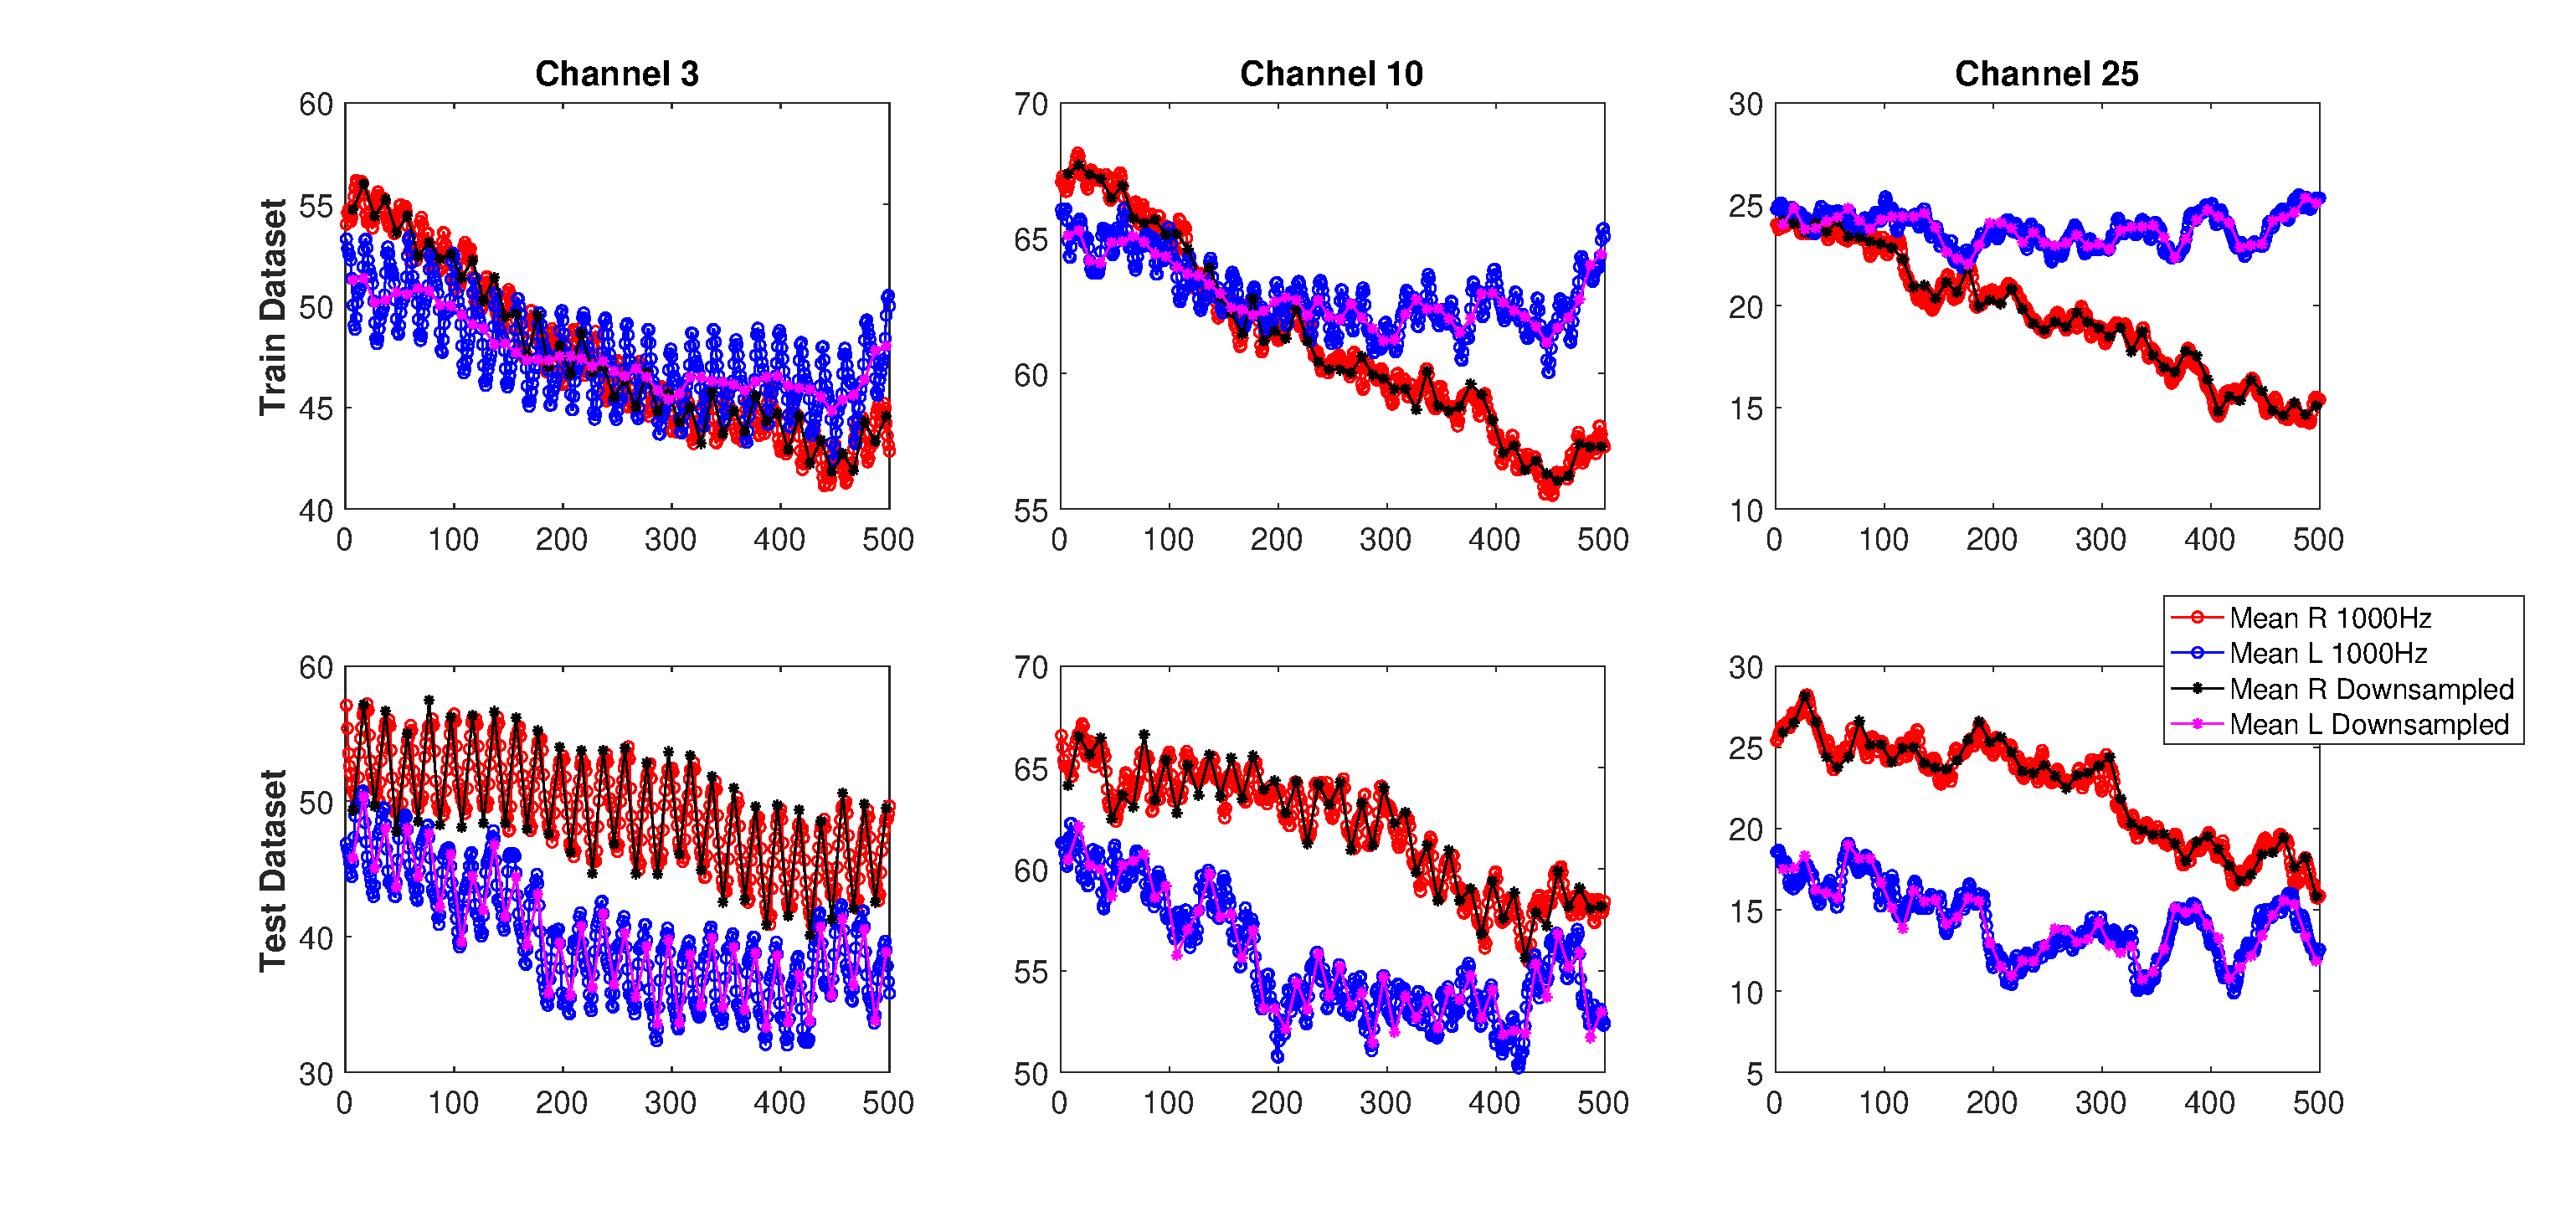
\includegraphics[width=1\textwidth]{fig/fig4new_mean_downsampled_vs1000} 
  \caption{Comparison of training and test datasets averages per channel over 316 and 100 samples, respectively.  
  Three channels (i.e., 3, 10 and 25) are randomly chosen, but the results generalise to all. 
  Each plot shows the mean of the samples with output 0 (i.e., classified as ``right'') and those with output 1 (i.e., classified as ``left''). 
For some channels (e.g., channel 3) the down-sampled averages present a lower variability than those sampled at higher resolution. 
  In all cases, the averages of the training set are distinctively different from those of the test set. 
  \label{fig_mean_1000hz_vs_downsampled}}
  \end{center}
  \end{figure}
  % End of Fig1
 To support this idea, Figure \ref{fig_fewsamples_vs_mean_downsampled}  shows the behaviour of three randomly chosen samples with frequency 100 Hz for each class (i.e., left and right) for both the training and test dataset. 
 Immediately, we can see that both the training and test selected samples are all very noisy and distant from their corresponding average.
 As expected, we can not recognize a pattern for the signals corresponding to the left or right classification. 
 %Fig2
  \begin{figure}[t]
 \begin{center}
  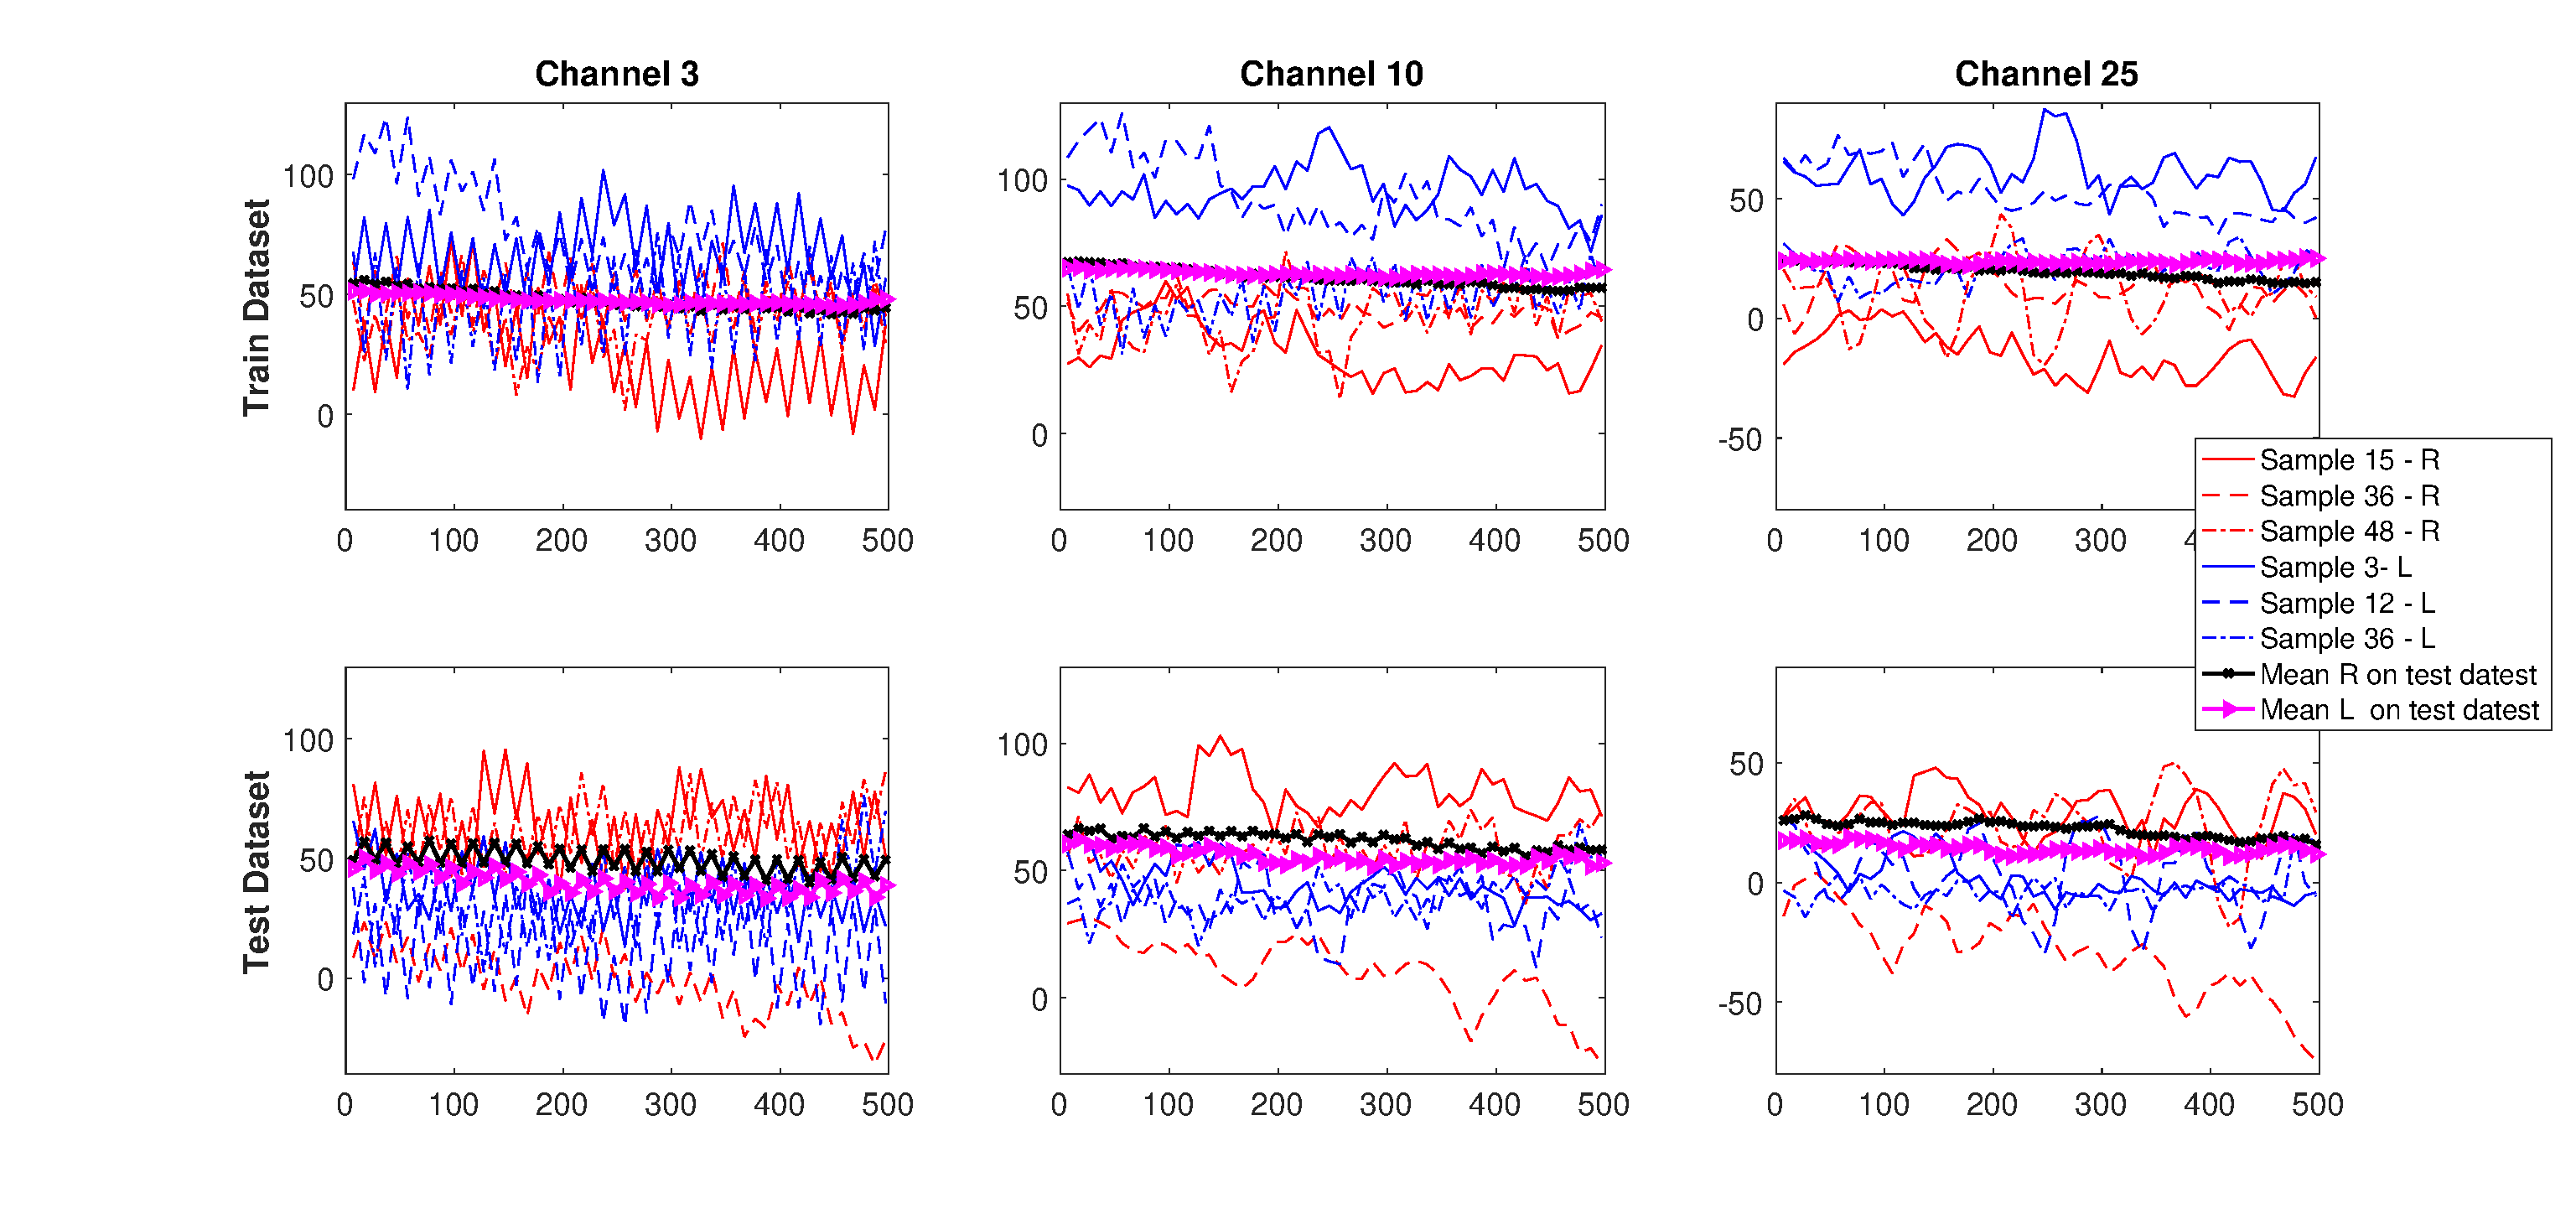
\includegraphics[width=1\textwidth]{fig/fig5new_fewsamples_mean_downsampled} 
  \caption{Plot of few randomly chosen samples from training and test datasets for channels 3, 10 and 25.
  Samples classified as 0 (i.e., ``right'') are plotted in red, while   samples classified as 1 (i.e., ``left'') are plotted in blue.
  \label{fig_fewsamples_vs_mean_downsampled}}
  \end{center}
  \end{figure}
  % End of fig2

Finally, driven by the results already published for this dataset \cite{bci_ii} and supported by other studies (see e.g. \cite{schirrmeister2017deep}), we propose a pre-processing strategy to reduce both the generalisation error and the size of the model needed to fit the training set.
Indeed, by reducing the noise in the data, i.e., by increasing the signal-to-noise ration, we aim at reducing the amount of variation that the model has to take into account and thus hope that a simpler model can better classify our data  \cite{goodfellow2016deep} . 
A \emph{filtering preprocessing} technique is therefore applied to our  final model, as explained in Section \ref{sec_themodel}.
In particular, we use the 1D Savitzky-Golay filter \cite{savgol} to smooth the data without greatly distorting the signal. 
By a convolution, the filter fits successive subsets of adjacent data points in a low-degree polynomial using the linear least squares method. 
In our tests, we use subsets of 7 points to be fitted in a polynomial of order 3. 


 

 % All models + data aug 
 \section{Considered models}\label{sec_allmodel}
 In this section, we describe some of the models we tested on the EEG signals and summarise their performance in terms of percentage error on a validation dataset. 
 Each of these models is tested using both the standard down-sampled dataset of size 316 and an \emph{augmented dataset}. 
 The latter is obtained by pre-processing the dataset to reduce the generalisation error \cite{goodfellow2016deep}. 
 In particular, we exploit the 1000~Hz dataset to extract not one, but 10  signals with frequency 100 Hz. 
Clearly, each of these signals will start at time $i$ with $i=0,\dots,9$. 
However, we believe that  issues cause by this mis-alignment can be neglected. 
In this way, the training dataset has the following dimensions: 3160 samples, 28 channels and 50 time-steps. 
% Remark: only on training - you cant augment the test and take some of those in the training, it'd be too simple

In the following, we provide a small description of each model we considered.
The diagrams representing the graph structures show the dimensions of the input and output tensors of each module composing the networks except for the non-linear nodes because they do not modify the dimensionality of the inputs.
In all diagrams, $n$ is the number of input samples.
For all models,    in order to reduce the discrepancies, we  normalise the training dataset using its mean and standard deviation for all channels. 
  The same values are used to normalise the test and cross-validation datasets. 

\begin{itemize}
\item \textbf{Linear perceptron (M1).} 
The simplest model one could devise for a classification problem is the linear perceptron:  given an input tensor $x$, the output is computed by the model as $y_{ij} = \sum_{k}x_{ik} A_{jk} + b_{j}$, where $A$ is the matrix of weights, and $b$ is the bias vector.

\item \textbf{Simple convolutional linear network (M2).} 
We consider two convolutional layers, both  combined with average pooling and ReLU non-linearities and then followed by two additional linear layers. 
The kernels are moved in the direction of the time-steps.
\begin{figure}[H]
\centering
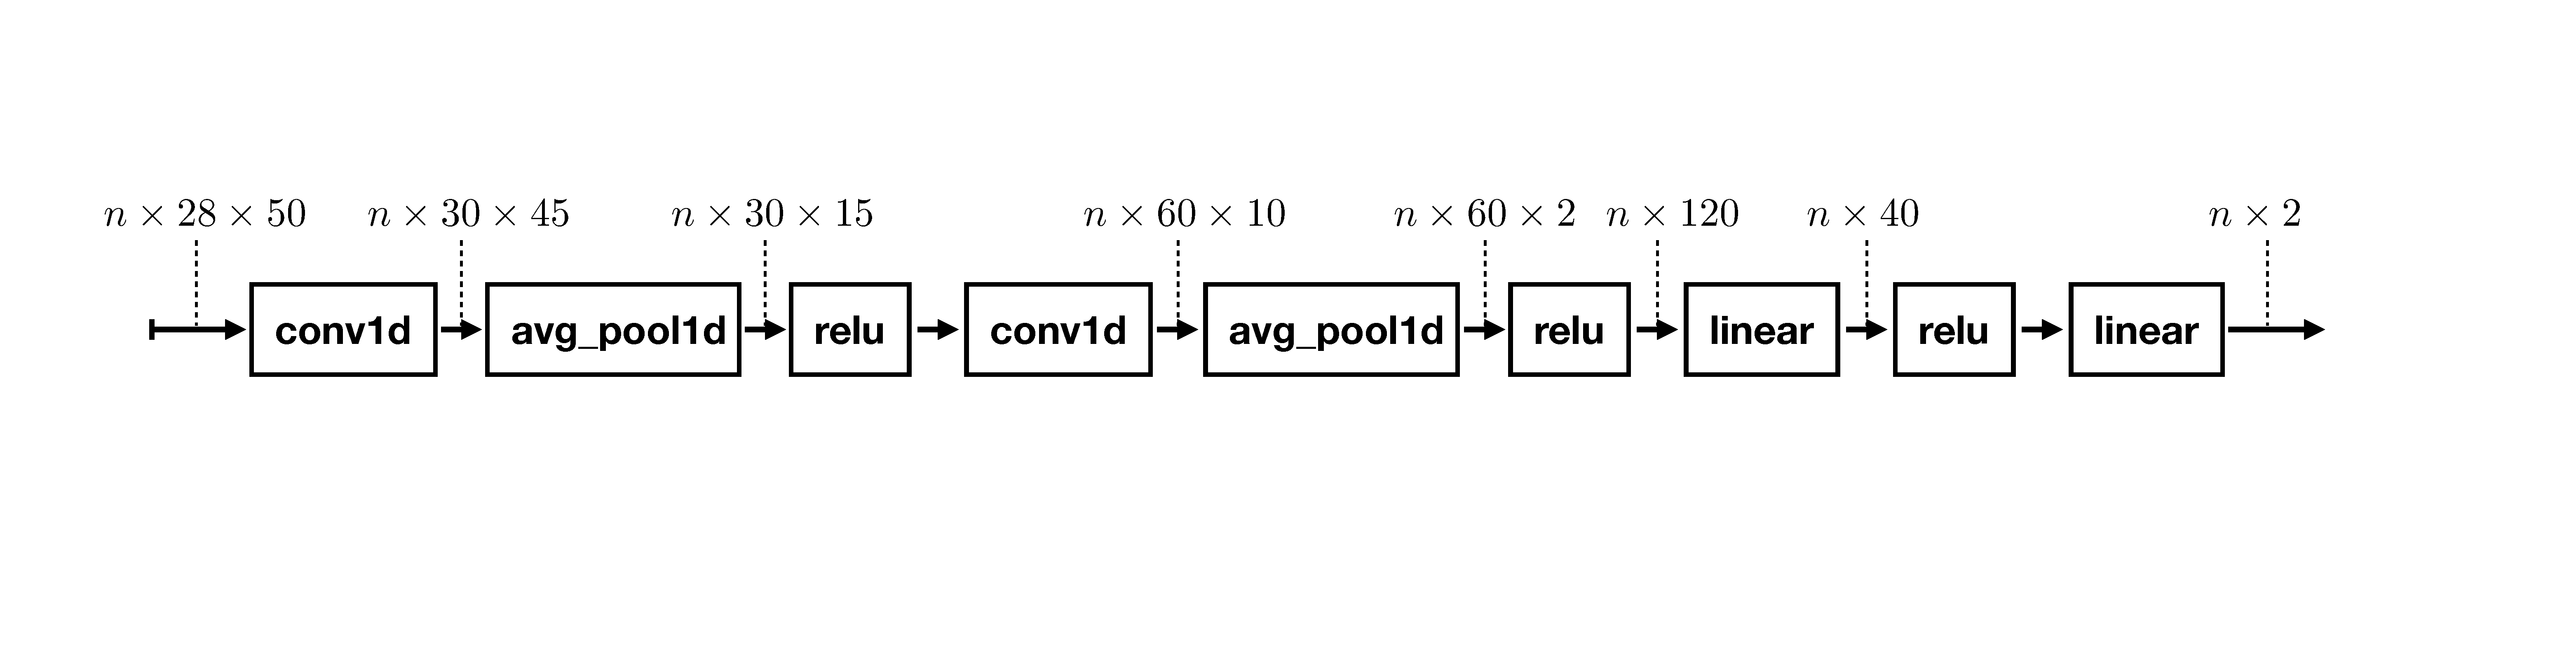
\includegraphics[width=\textwidth, clip=true,trim=100 300 295 230]{fig/conv1.pdf}
\end{figure}

\item \textbf{Multichannel deep convolutional neural network + linear perceptron (M3).}
The convolutional layer in this model is such that  different masks are applied to each channel; at the implementation level, this is achieved by setting the \verb|groups| parameter equal to 28 in the constructor of the model. Convolutions of this kind are employed to study  uni-dimensional time-series multichannel also in \cite{zheng2014time}.
\begin{figure}[H]
\centering
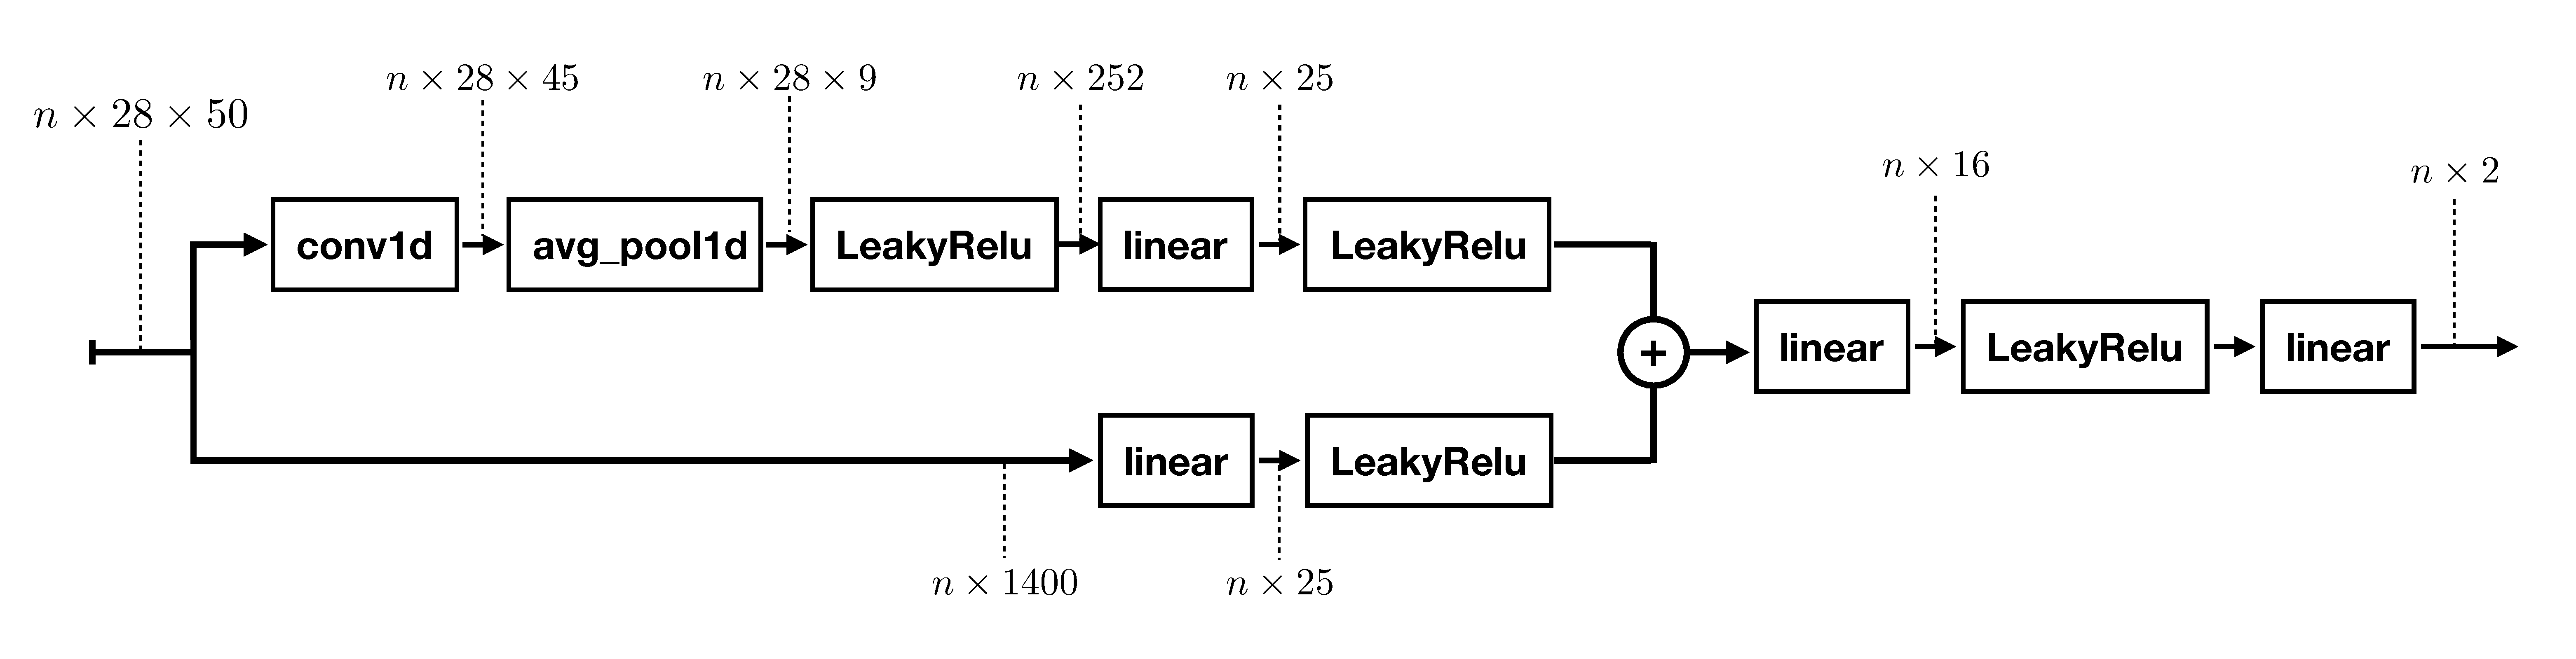
\includegraphics[width=\textwidth, clip=true,trim=30 40 70 50]{fig/conv2.pdf}
\end{figure}

\item \textbf{Shallow convolutional neural network (M4).}
In this network, the first and the second convolutions operate in the dimension of the time-steps and the channels, respectively. 
We took inspiration from \cite{schirrmeister2017deep} for the design of this model.
\end{itemize}
\begin{figure}[H]
\centering
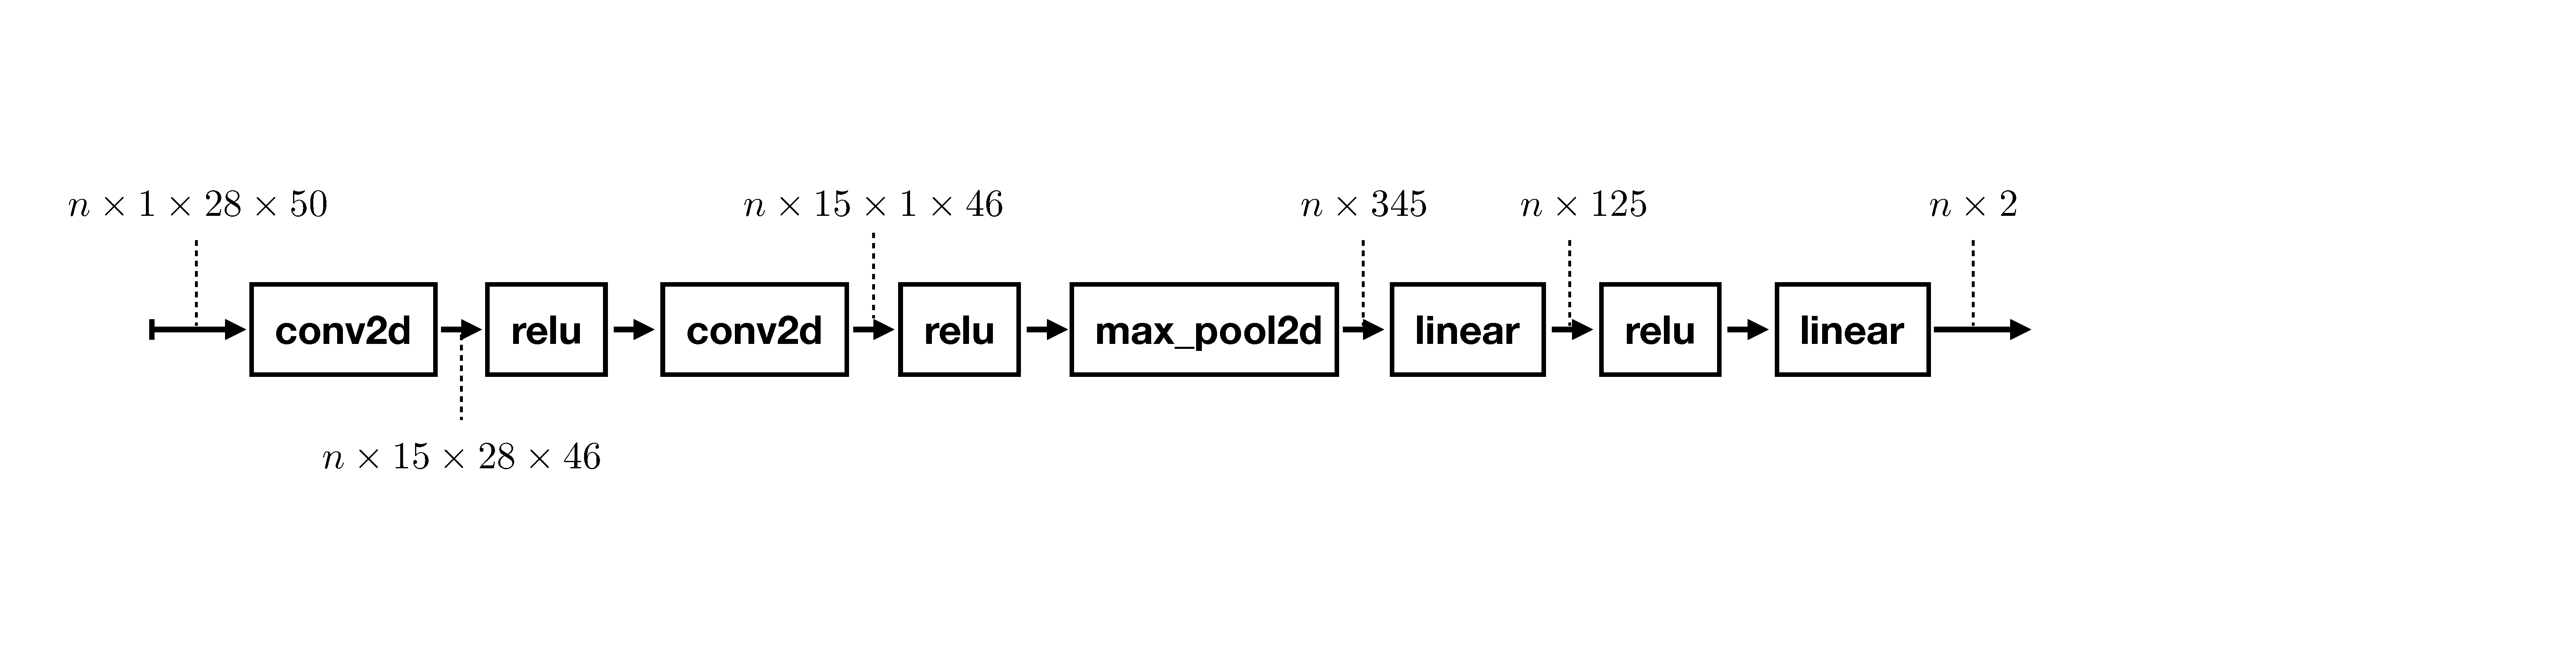
\includegraphics[width=\textwidth, clip=true,trim=80 200 520 200]{fig/conv3.pdf}
\end{figure}


%The models are tested on the standard down-sampled and augmented datasets to evaluate their performance.  % -- RIPETIZIONE (VEDI INIZIO SEZIONE)

% Comments on the architecture and optimisation step 
We use the stochastic ADAM for the optimisation step, with bash size equal to 100 or to 1000  for the standard and augmented training datasets, respectively. 
The learning rate $\varepsilon$ is equal to  $10^{-1}$ for the linear perceptron and $10^{-3}$ for the other three models. 
This choice is made  for convergence purposes. 
The models are optimised according to the cross entropy loss function. 

% Results
Table~\ref{tab_results} shows the performance of the four models in terms of percentage error on a cross-validation dataset (obtained by randomly choosing 10\% of the samples of the train dataset) after 1000 epochs of the stochastic gradient descent (SGD). 
Each model is run 10 times and the variability in the results is due to the random initialisation of parameters and the SGD.
Surprisingly, the linear perceptron (M1) performs better than (M2) and (M3), leading to a smaller average error and variance. 
In the non-augmented dataset, however, the model that ensures a smaller minimum error and a smaller error on average is the shallow convolutional neural network (M4).

% Table1
 \begin{table}[h]
 \begin{center}
    \begin{tabular}{ l l l l l l l l l}
\toprule
     $ $ & \multicolumn{4}{c}{non-augmented dataset} & \multicolumn{4}{c}{augmented dataset} \\
     \cmidrule(lr){2-5}
     \cmidrule(lr){6-9}
   % Trial & M1 & M2 & M3 & M4 & M1 & M2 & M3 & M4  \\
     & M1 & M2 & M3 & M4 & M1 & M2 & M3 & M4  \\
\midrule
%    1 & 27 & 34 & 32 & 32 & 23 & 37 & 36 & 35 \\
%    2 & 27 & 29 & 33 & 25 & 24 & 32 & 36 & 37 \\
%    3 & 29 & 28 & 30 & 24 & 24 & 33 & 35 & 34\\
%    4 & 30 & 23 & 29 & 29 & 24 & 34 & 37 & 34\\
%    5 & 26 & 28 & 30 & 33 & 26 & 30 & 34 & 33\\
%    6 & 27 & 29 & 32 & 26 & 26 & 33 & 40 & 33\\
%    7 & 26 & 29 & 33 & 29 & 25 & 31 & 34 & 32\\
%    8 & 27 & 27 & 29 & 21 & 24 & 32 & 44 & 29\\
%    9 & 29 & 31 & 30 & 29 & 24 & 32 & 39 & 37 \\
%    10 & 26 & 32 & 31 & 22 & 24 & 32 & 36 & 35\\
%    \midrule
    Best & 26 & 23 & 28 & 21 & 23 & 28 & 34 & 29 \\
    Average & 27.4 & 29.0 & 30.9 & 27.0 & 24.4 & 32.6 & 37.1 & 32.9 \\
\bottomrule
    \end{tabular}
        \caption{Validation percentage errors for the linear perceptron (M1), the simple convolutional linear network (M2), the multichannel deep CNN combined with the linear perceptron (M3) and the shallow CNN (M4) using the down-sampeld set or the augmented one.\label{tab_results}}
\end{center}
\end{table}
% end table1

% Augmented dataset is not so good
Augmenting the dataset leads to a slightly smaller error for M1, but to a considerable loss of accuracy for the other three models. 
We suppose that, with a different choice of parameters (e.g., size of convolutional and pool nodes, kernels), the advantage of using a larger datasets could be exploited also for M2, M3 and M4. 

% Remark
Since the shallow convolutional network (M4) showed the most promising results in these primarily test runs, in the following section we focus on optimising this particular network. 
It is important to notice that our results  are greatly determined by the choices of parameters for each of the networks we considered; it is possible that other combinations for M2 and M3 could lead to smaller errors.


% Section - hyperparam
  \section{Further investigation of CNN model}\label{sec_themodel}
\subsection{Overfitting}
 The validation error, as function of the number of epochs, shows the typical U-shape (i.e., the  validation error slowly grows after reaching a minimum) which implies  that the considered models are affected by overfitting \cite{goodfellow2016deep}. 
 Additionally, we observe a  significant difference between the models performances on the train and validation sets, i.e. the train percentage error is much lower than the cross-validation percentage error, which confirms the overfitting hypothesis. 
Although the substantial noise  in the datasets is probably the main cause behind overfitting, we have adopted different strategies to solve this problem. 
First, by manually tuning the sizes of the linear layers in M4, we observe that they play an important role in terms of overfitting and the best results are obtained when the number of neurons lies in the interval $[100,150]$. 
This interval is optimal as it takes into account a direct tradeoff between overfitting and model complexity: smaller layers  than the ones in the prescribed interval are not accurate enough and larger layers lead to an even  more evident overfitting effect. 
The second approach consists in the addition of a parameter penalty norm $L_2$, which is obtained by passing the penalty constant to the optimiser object of the Pytorch library. 
Finally, dropout layers are introduced before linear layers to prevent complex co-adaptions and hence giving a network that generalises better.


\subsection{Hyper-parameter optimisation}
After identifying  the most promising model in Section \ref{sec_allmodel} and choosing the  regularisation strategy, we procede with hyper-parameters optimisation to further improve the performance of the network (see \verb|hyperoptimization.py| for the implementation). 
 Given the shortage of available computational resources, we adopted a random search approach for the exploration of the parameter space using an initial ansatz  on the lower- and upper-bound of each parameter.
 Additionally,  these initial guessed intervals are regularly updated.
 On the one hand, when we observe that for parameters too close to boundaries we do not reach convergence, we reduce the interval spread.
 On the other hand, if we notice that for parameters close to one either the lower- or the upper-bounds the accuracy is high, we modify the bounds to include smaller or higher values, respectively. 

We consider three groups of  parameters (architecture, training and regularisation) and their intervals, chosen after few refinement steps, are listed in Table~\ref{tab_hyperparam_optim}.  
 Architecture parameters are related to capacity of the network and control the size of weights and biases of hidden layers.
 As mentioned in the previous section, the ADAM algorithm is adopted to optimise the network with a stochastic mini-batch procedure to update the weights and biases. 
Moreover,  instead of considering a constant learning rate $\varepsilon$, we adopt a geometric progression: the initial learning rate $\varepsilon_0$ is multiplied by the scaling rate $d$ once every 30 epochs. 
The  mini-batch size  together with $\varepsilon$ and $d$ are the training   hyper-parameters we aim at optimising. 
Finally, regarding regularisation, both the dropout probability and the $L_2$ penalty constant are treated as hyper-parameters.
 
 
% table 2
\begin{table}
  \begin{center}
    \begin{tabular}{ c c c }
      \toprule
        \multicolumn{1}{c}{{Group}} & \multicolumn{1}{c}{{Type}} & \multicolumn{1}{c}{{Interval}}  \\
       \midrule
       \multirow{4}{*}{\makecell{Architecture \\ parameters}} & Output channels: First convolution & $[10,80]$ \\
        & Output channels: Second convolution & $[10,80]$ \\
        & Kernel size: First convolution & $[3,13]$  \\
        & Output size: Hidden linear layer & $[100,150]$ \\ \midrule
        \multirow{3}{*}{\makecell{Training \\ parameters}} & Initial learning rate $\varepsilon$& $[10^{-5},10^{-2}]$\\
        & Scaling rate $d$ & $[0.7,0.95]$  \\
        & Batch size $\%$ & $[10,50]$ \\ \midrule
        \multirow{2}{*}{\makecell{Regularization \\ parameters}} & Dropout probability & $[0.2,0.5]$   \\
        & $L_2$ penalty constant & $[10^{-6},10^{-1}]$   \\
\bottomrule
    \end{tabular}
        \caption{Intervals  for each parameter adopted in the hyper-parameter optimisation step. The reported intervals are the result of an  initial educated guess, which has then be refined when we noticed that for some too large or too small values convergence was not obtained. \label{tab_hyperparam_optim}}
\end{center}
\end{table}
% end table two


This set of 9  hyper-parameters is used for optimisation in three different scenarios: 
\begin{itemize}
\item the \emph{regular dataset}, i.e. the down-sampled one with $50$ time-steps per channel; 
\item the \emph{augmented dataset} described in the previous section;% obtained starting from the regular dataset and enriching it with  repeated down-samplings of the larger dataset.
\item the \emph{smoothed dataset} obtained  by applying the smoothing filter described at the end of Section~\ref{sec_visual}.
\end{itemize}
For all scenarios, we sample uniformly from the intervals given in Table~\ref{tab_hyperparam_optim} and, after 1000 runs we select the set of parameters which provides the smallest cross-validation error when using the 90\% of regular dataset as training set and 10\% as validation set.
In this scenario, we obtained the smallest validation error equal to 12.9\%  when the following set of parameters is used:
Batch size $ =  0.3$,  Initial learning rate $\varepsilon  = 0.001$,  Output channels - First convolution  $= 14$, Output channels - Second convolution $= 35$, Kernel size - First convolution $= 3$, Output size: Hidden linear layer $ = 105$,  Scaling rate $d = 0.897$, Dropout probability $=  0.313$,  $L_2$ penalty constant $= 1.416$e-05.
Finally, in order to test this model on the test set, we consider an empty cross validation set (i.e., the full training set is used in the training part) and, after running this model 100 times, we obtain our best result  28\% error on the test set.
This result is not very satisfactory, but we suppose that this is due to the poor dataset and its discrepancies between train and test sets. 
 Moreover, we observe that the random initialisation of parameters and SGD plays a big role in the final output. 
Choosing larger cross-validation set or using  the other two scenarios (augmented  and smoothed sets), result in worse outcomes. 
  
  % Conclusion
 \section{Conclusion}\label{sec_conclusion}
 We proposed a CNN model to classify  EEG data to predict a binary choice, which was chosen out of four  increasingly complex models as the one which provided the smallest error on the cross-validation set. 
 On this model, we run hyper-parameter optimisation to find its best architecture and the best choice of parameters with respect to the validation set error. For a particular choice of parameters, we manage to obtain a 12.9\% validation error. The same parameters are then used over 100 runs of the model in which no validation is performed: here, our best result on test set has an accuracy of 72\% and on average we obtain an accuracy of 70\%. 
 Nevertheless,  even if we understand that this is not the correct reasoning to follow, we tried to find the best hyper-parameters for the test set.  For the following setting we obtain an accuracy of 82\% on the test set. The model is stored in the best\_model/ folder in the root of the project, and a forward pass of the best model we found can be executed by running the \verb|run_forward_of_best_model.py| script in the root of the project.
 The hyper-parameters in this case are:
 Batch size $ =  0.191$,  Initial learning rate $\varepsilon  = 0.001$,  Output channels - First convolution  $= 18$, Output channels - Second convolution $= 12$, Kernel size - First convolution $= 11$, Output size: Hidden linear layer $ = 122$,  Scaling rate $d = 0.9$, Dropout probability $=  0.35$,  $L_2$ penalty constant $=0.001$.

 To conclude, we believe that the proposed framework and the subsequent choices we made could have performed better if the initial dataset was less noisy or more numerous. The regularisation strategies we adopted did not significantly improve the model; additional approaches we wished we had time to test are the early stopping, the noisy labels and the add of random noise to the training set. Nevertheless, by performing the hyper-parameter optimization we managed to achieve a slight improvement with respect to the initial chosen model in terms of validation and test error.
 
 % References
\bibliographystyle{abbrv}
\bibliography{mybib_dl} 
  
  
  
\end{document}